\subsection{Modules over a local ring}

PROPOSITION 4. Let A be a ring which is not necessarily commutative, m a right ideal of A contained in the Jacobson radical of A and M a left A-module. Suppose that one of the following conditions holds:

\begin{enumerate}
\def\labelenumi{(\roman{enumi})}
\item
  M is finitely generated;
\item
  m is nilpotent.
\end{enumerate}

Then the relation \((\mathbf{A}_d / \mathfrak{m})\otimes_{\mathbf{A}}\mathbf{M} = 0\) implies \(\mathbf{M} = 0\)

The assertion with respect to hypothesis (i) is precisely Corollary 3 to Proposition 6 of Algebra, Chapter VIII, § 6, no. 3. On the other hand, the relation \((\mathbf{A}_d / \mathfrak{m}) \otimes_{\mathbf{A}} \mathbf{M} = 0\) is equivalent to \(\mathbf{M} = \mathfrak{m}\mathbf{M}\) and hence implies \(\mathbf{M} = \mathfrak{m}^n\mathbf{M}\) for every integer \(n > 0\) ; whence the assertion with respect to hypothesis (ii).

COROLLARY 1. Let A be a ring which is not necessarily commutative, m a right ideal of A contained in the Jacobson radical of A, M and N two left A-modules and u: M → N an A-linear mapping. If N is finitely generated or m is nilpotent and

\[
1 \otimes u: (A _ {d} / m) \otimes_ {A} M \rightarrow (A _ {d} / m) \otimes_ {A} N
\]

is surjective, then u is surjective.

\((\mathbf{A}_d / \mathfrak{m})\otimes_{\mathbf{A}}(\mathbf{N} / u(\mathbf{M}))\) is canonically isomorphic to

\[
((\mathrm{A} _ {d} / \mathfrak {m}) \otimes_ {\mathrm{A}} \mathrm{N}) / \operatorname{Im} (1 \otimes u)
\]

(Algebra, Chapter II, § 3, no. 6, Corollary 1 to Proposition 6); then the hypothesis implies \((\mathbf{A}_d / \mathfrak{m}) \otimes_{\mathbf{A}} (\mathrm{N} / u(\mathbf{M})) = 0\) , hence \(\mathrm{N} / u(\mathbf{M}) = 0\) by Proposition 4.

COROLLARY 2. Let A be a ring which is not necessarily commutative, m a two-sided ideal of A contained in the Jacobson radical of A, M a left A-module and \((x_{\iota})_{\iota \in I}\) a family of elements of M. If M is finitely generated or m is nilpotent and the elements \(1 \otimes x_{\iota} (\iota \in I)\) generate the left (A/m)-module (A/m) \(\otimes_{\mathbf{A}} \mathbf{M}\) , the \(x_{\iota}\) generate M.

Let \((e_t)_{t \in I}\) be the canonical basis of the left A-module \(\mathbf{A}_s^{(I)}\) : it is sufficient to apply Corollary 1 to the A-linear mapping \(u: \mathbf{A}_s^{(I)} \to \mathbf{M}\) such that \(u(e_t) = x_t\) for all \(t \in I\) .

PROPOSITION 5. Let A be a ring which is not necessarily commutative, m a two-sided ideal of A contained in the Jacobson radical of A and M a left A-module. Suppose that one of the following conditions holds:

\begin{enumerate}
\def\labelenumi{(\roman{enumi})}
\item
  M is finitely presented;
\item
  m is nilpotent.
\end{enumerate}

Then, if \((\mathbf{A} / \mathfrak{m})\otimes_{\mathbf{A}}\mathbf{M} = \mathbf{M} / \mathfrak{m}\mathbf{M}\) is a free left \((\mathbf{A} / \mathfrak{m})\) -module and the canonical homomorphism from \(\mathfrak{m}\otimes_{\mathbf{A}}\mathbf{M}\) to \(\mathbf{M}\) is injective, \(\mathbf{M}\) is a free A-module. To be precise, if \((x_{t})_{t\in I}\) is a family of elements of \(\mathbf{M}\) such that \((1\otimes x_{t})\) is a basis of the \((\mathbf{A} / \mathfrak{m})\) -module \(\mathbf{M} / \mathfrak{m}\mathbf{M}, (x_{t})\) is a basis of \(\mathbf{M}\) .

If \(a \in \mathbf{A}\) , \(x \in \mathbf{M}\) and \(\bar{a}\) is the class of \(a\) in \(\mathbf{A} / \mathfrak{m}\) , then \(\bar{a} \otimes x = 1 \otimes (ax)\) and hence the hypothesis implies that there exists a family \((x_{t})_{t \in I}\) of elements of \(\mathbf{M}\) such that \((1 \otimes x_{t})\) is a basis of the \((\mathbf{A} / \mathfrak{m})\) -module \((\mathbf{A} / \mathfrak{m}) \otimes_{\mathbf{A}} \mathbf{M}\) . We already know that the \(x_{t}\) generate \(\mathbf{M}\) (Corollary 2 to Proposition 4); we shall see that they are linearly independent over \(\mathbf{A}\) . To this end, let us consider the free A-module \(\mathbf{L} = \mathbf{A}_{s}^{(\mathrm{I})}\) ; let \((e_{t})\) be its canonical basis and \(u: \mathbf{A}_{s}^{(\mathrm{I})} \to \mathbf{M}\) the A-linear mapping such that \(u(e_{t}) = x_{t}\) for all \(t \in I\) ; if \(R\) is the kernel of \(u\) , we shall prove that \(R = 0\) . Under hypothesis (i), \((\mathbf{A} / \mathfrak{m}) \otimes_{\mathbf{A}} M\) is a finitely generated \((\mathbf{A} / \mathfrak{m})\) -module, hence \(I\) is necessarily finite and \(R\) is a finitely generated A-module by Chapter I, § 2, no. 8, Lemma 9. Then by Proposition 4 it will be sufficient to prove (under either hypothesis) that \(R = mR\) .

Let \(j\) be the canonical injection \(\mathbf{R} \to \mathbf{L}\) ; then there is a commutative diagram

\[
\begin{array}{c c c c c} \mathfrak {m} \otimes \mathrm{R} & \xrightarrow {1 \otimes j} & \mathfrak {m} \otimes \mathrm{L} & \xrightarrow {1 \otimes u} & \mathfrak {m} \otimes \mathrm{M} \\ a \Big \downarrow & & b \Big \downarrow & & c \Big \downarrow \\ \mathrm{R} & \xrightarrow {} _ {j} & \mathrm{L} & \xrightarrow {} _ {u} & \mathrm{M} \end{array}
\]

in which the two rows are exact, \(j\) is injective and \(1 \otimes u\) is surjective (Chapter

I, §2, no. 1, Lemma 1); as, by hypothesis, \(\operatorname{Ker}(c) = 0\) , there is an exact sequence

\[
0 \xrightarrow {d} \operatorname{Coker} (a) \longrightarrow \operatorname{Coker} (b) \xrightarrow {v} \operatorname{Coker} (c)
\]

(Chapter I, § 1, no. 4, Proposition 2); it is sufficient to verify that \(v\) is bijective, for then we deduce that \(\operatorname{Coker}(a) = 0\) , in other words that \(a\) is surjective and consequently \(\mathbf{R} = \mathfrak{m}\mathbf{R}\) . Now, \(\operatorname{Coker}(b) = (\mathbf{A}/\mathfrak{m}) \otimes_{\mathbf{A}} \mathbf{L}\) and

\[
\operatorname{Coker} (c) ^{\prime} = (\mathrm{A} / \mathfrak {m}) \otimes_ {\mathrm{A}} \mathrm{M}
\]

and by definition \(v(1 \otimes e_t) = 1 \otimes x_t\) ; as \((1 \otimes e_t)\) is a basis of \((\mathbf{A} / \mathfrak{m}) \otimes_{\mathbf{A}} \mathbf{L}\) , the definition of the \(x_t\) shows that \(v\) is bijective.

COROLLARY 1. Let A be a not necessarily commutative ring, m the Jacobson radical of A and M a left A-module. Suppose that A/m is a field, that the canonical homomorphism from m ⊗A M to M is injective and that one of conditions (i), (ii) of Proposition 5 is satisfied. For a family (yλ) of elements of M to be a basis of a direct factor of M, it is necessary and sufficient that the family (1 ⊗yλ) be free in M/mM.

If this condition holds, it can be assumed that \((y_{\lambda})\) is a subfamily of a family \((x_{t})\) of elements of M such that \((1 \otimes x_{t})\) is a basis of M/mM (Algebra, Chapter II, §7, no. 1, Theorem 2) and Proposition 5 then proves that \((x_{t})\) is a basis of M.

COROLLARY 2. Let A be a not necessarily commutative ring, m the Jacobson radical of A and M a left A-module. Suppose that A/m is a field and that one of the following conditions holds:

\begin{enumerate}
\def\labelenumi{(\roman{enumi})}
\item
  M is finitely presented;
\item
  m is nilpotent.
\end{enumerate}

Then the following properties are equivalent:

\begin{enumerate}
\def\labelenumi{(\alph{enumi})}
\item
  M is free;
\item
  M is projective;
\item
  M is flat;
\item
  the canonical homomorphism \(\mathfrak{m} \otimes_{\mathbf{A}} \mathbf{M} \to \mathbf{M}\) is injective;
\end{enumerate}

* (e) \(\mathrm{Tor}_1^{\mathbf{A}}(\mathbf{A} / \mathfrak{m},\mathbf{M}) = 0.\) *

The implications (a) \(\Rightarrow\) (b) \(\Rightarrow\) (c) \(\Rightarrow\) (d) are immediate. As A/m is a field, (A/m) \(\otimes_{\mathrm{A}} \mathrm{M}\) is a free (A/m)-module and Proposition 5 shows that (d) implies (a).

* Finally, we know that \(\operatorname{Tor}_1^{\mathbf{A}}(\mathbf{A},\mathbf{M}) = 0\) and from the exact sequence \(0\to \mathfrak{m}\to \mathbf{A}\to \mathbf{A} / \mathfrak{m}\to 0\) we therefore derive the exact sequence

\[
0 \rightarrow \operatorname{Tor} _ {1} ^ {\mathbf {A}} (\mathrm{A} / \mathfrak {m}, \mathrm{M}) \rightarrow \mathfrak {m} \otimes_ {\mathbf {A}} \mathrm{M} \rightarrow \mathrm{M};
\]

this proves that \(\operatorname{Tor}_1^{\mathbf{A}}(\mathbf{A} / \mathfrak{m},\mathbf{M})\) is isomorphic to the kernel of the canonical homomorphism \(\mathfrak{m}\otimes_{\mathbf{A}}\mathbf{M}\to \mathbf{M}\) ; whence the equivalence of (d) and (e). *

It can be shown that, for every ring A with Jacobson radical m such that A/m is a field, every projective A-module is free (Exercise 3).

PROPOSITION 6. Let A be a ring which is not necessarily commutative and m its Jacobson radical; suppose that A/m is a field. Let M and N be two finitely generated free A-modules and u: M → N a homomorphism. The following properties are equivalent:

\begin{enumerate}
\def\labelenumi{(\alph{enumi})}
\item
  \(u\) is an isomorphism of \(\mathbf{M}\) onto a direct factor of \(\mathbf{N}\) ;
\item
  \(1 \otimes u: (\mathbf{A} / \mathfrak{m}) \otimes_{\mathbf{A}} \mathbf{M} \to (\mathbf{A} / \mathfrak{m}) \otimes_{\mathbf{A}} \mathbf{N}\) is injective;
\item
  \(u\) is injective and \(\operatorname{Coker}(u)\) is a free A-module;
\item
  the transpose homomorphism \(^{t}u: N^{*} \rightarrow M^{*}\) is surjective.
\end{enumerate}

We know (Algebra, Chapter II, § 1, no. 11, Proposition 21) that, if N/u(M) is free, u(M) is a direct factor of N, hence (c) implies (a); conversely, (a) implies that Coker(u), isomorphic to a complement of u(M) in N, is a finitely generated projective A-module and a fortiori finitely presented (Chapter I, § 2, no. 8, Lemma 8); hence this module is free by Corollary 2 to Proposition 5 and (a) implies (c). On the other hand, (a) obviously implies (b). For simplicity we write M' = (A/m) ⊗\_A M, N' = (A/m) ⊗\_A N; as M and N are finitely generated, the duals M'* and N'* of the (A/m)-modules M' and N' are canonically identified with M* ⊗\_A (A/m) and N* ⊗\_A (A/m) and t(1 ⊗ u) with (t u) ⊗ 1 (Algebra, Chapter II, § 5, no. 4, Proposition 8); as M' and N' are vector spaces over the field A/m, the hypothesis that 1 ⊗ u is injective implies that t(1 ⊗ u) is surjective (Algebra, Chapter II, § 7, no. 5, Proposition 10); Corollary 1 to Proposition 4 then shows that t u is surjective and we have thus proved that (b) implies (d). Finally we show that (d) implies (a). Suppose that t u is surjective; as M* is free, there exists a homomorphism f from M* to N* such that l\_M* = t u ∘ f (Algebra, Chapter II, § 1, no. 11, Proposition 21); as M and N are free and finitely generated, there exists a homomorphism g from N to M such that f = t g; hence t l\_M = l\_M* = t u ∘ t g = t(g ∘ u), whence l\_M = g ∘ u; this proves that u is an isomorphism of M onto a submodule which is a direct factor of N (Algebra, Chapter II, § 1, no. 9, Corollary 2 to Proposition 15).

COROLLARY. Under the hypotheses of Proposition 6 the following properties are equivalent:

(a) \(u\) is an isomorphism of \(\mathbf{M}\) onto \(\mathbf{N}\) ;

(b) \(M\) and \(N\) have the same rank (Algebra, Chapter II, § 7, no. 2) and \(u\) is surjective;

(c) \(1 \otimes u: M/\mathfrak{m}M \to N/\mathfrak{m}N\) is bijective.

Clearly (a) implies (b); (b) implies that \(1 \otimes u\) is surjective; moreover the hypothesis that M and N have the same rank implies that so do the vector spaces \((\mathrm{A} / \mathfrak{m}) \otimes_{\mathbf{A}} \mathbf{M}\) and \((\mathrm{A} / \mathfrak{m}) \otimes_{\mathbf{A}} \mathbf{N}\) over \(\mathrm{A} / \mathfrak{m}\) , hence \(1 \otimes u\) is bijective (Algebra, Chapter II, § 7, no. 4, Corollary to Proposition 9) and (b) implies (c). Finally, condition (c) implies, by Proposition 6, that N is the direct sum of \(u(\mathbf{M})\) and a free submodule P and \(u\) is an isomorphism of M onto \(u(\mathbf{M})\) ; if \(\mathrm{P} \neq 0\) , then \((\mathrm{A} / \mathfrak{m}) \otimes_{\mathbf{A}} \mathrm{P} \neq 0\) and \(1 \otimes u\) would not be surjective; hence (c) implies (a).

The propositions proved above in this no. will usually be applied when A is a local ring and m its maximal ideal. Corollary 2 to Proposition 5 is then completed by

PROPOSITION 7. Let A be a reduced local ring, m its maximal ideal, \((\mathfrak{p}_{\iota})_{\iota \in I}\) the family of minimal prime ideals of A, \(K_{\iota}\) the field of fractions of A/ \(p_{\iota}\) and M a finitely generated A-module. For M to be free it is necessary and sufficient that

\[
[ (\mathrm{A} / \mathfrak {m}) \otimes_ {\mathrm{A}} \mathrm{M}: (\mathrm{A} / \mathfrak {m}) ] = [ \mathrm{K} _ {\iota} \otimes_ {\mathrm{A}} \mathrm{M}: \mathrm{K} ] \quad \text{for all }\iota \in \mathrm{I}.\tag{1}
\]

If M is free, clearly the two sides of (1) are equal to the rank of M for all \(\iota\in I\) . Suppose now that the condition is satisfied and denote by n the common value of the two sides of (1); by Corollary 2 to Proposition 4 M has a system of n generators \(x_{j}\) ( \(1\leqslant j\leqslant n\) ). Suppose first that A is an integral domain, in which case \(p_{i}=0\) for all \(\iota\in I\) . The elements \(1\otimes x_{j}\) ( \(1\leqslant j\leqslant n\) ) generate the vector space \(K\otimes M\) over the field of fractions K of A; but as by hypothesis this space is of dimension n over K, the elements \(1\otimes x_{j}\) are linearly independent over K. It follows (Algebra, Chapter II, §1, no. 13, Remark 1) that the \(x_{j}\) are linearly independent over A and hence form a basis of M.

Passing to the general case, there exists a surjective homomorphism \(v\) from \(\mathbf{L} = \mathbf{A}^n\) onto \(\mathbf{M}\) . Consider the commutative diagram

\pandocbounded{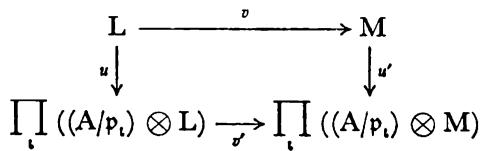
\includegraphics[keepaspectratio]{images/part001_964082be.jpg}}

where \(u\) (resp. \(u'\) ) is the mapping \(x \mapsto (\phi_{\iota}(x))\) (resp. \(y \mapsto (\psi_{\iota}(y)))\) ,

\[
\phi_ {i} \colon \mathbf {L} \rightarrow (\mathbf {A} / \mathfrak {p} _ {i}) \otimes \mathbf {L}
\]

(resp. \(\psi_{t}\colon\mathbf{M}\to(\mathbf{A}/p_{t})\otimes\mathbf{M}\) ) being the canonical mapping, and \(v'\) is the product of the \(1_{\mathbf{A}/p_{t}}\otimes v\) . Then \((\mathbf{A}/p)/(m/p_{t})\otimes_{\mathbf{A}/p_{t}}((\mathbf{A}/p_{t})\otimes_{\mathbf{A}}\mathbf{M})=(\mathbf{A}/m)\otimes_{\mathbf{A}}\mathbf{M}\) and, as \(A/p_{t}\) is a local integral domain, it follows from the first part of the argument that each of the \(1_{\mathbf{A}/p_{t}}\otimes v\) is an isomorphism; then so is \(v'\) . On the other hand, as A is reduced, \(\bigcap_{i} p_{i} = (0)\) ( \(\S 2\) , no. 6, Proposition 13), whence \(\bigcap_{i} (p_{i} L) = 0\) since L is free (Algebra, Chapter II, \(\S 3\) , no. 7, Remark); as \(p_{i} L\) is the kernel of \(\phi_{i}\) , this shows that \(u\) is injective. It follows that \(v' \circ u = u' \circ v\) is injective, hence \(v\) is injective and, as \(v\) is surjective by definition, this shows that M is free.

